\chapter{Functional Requirements}
\label{chap:functional}

Requirements are identified with the prefix \textbf{FR-} (Functional Requirement).
Priority levels: \textbf{M} = Must Have, \textbf{S} = Should Have,
\textbf{C} = Could Have.

% ─────────────────────────────────────────────────────────────────────────────
\section{Feature 1: Host Input and Scan Initiation}
\label{sec:fr_input}

\begin{figure}[H]
  \centering
  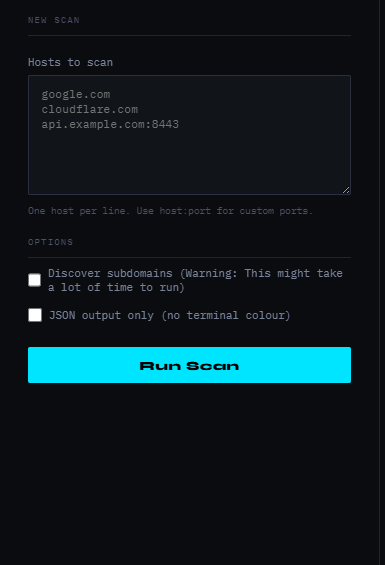
\includegraphics[width=0.55\textwidth]{images/web_input.png}
  \caption{Web GUI — Input panel with host list and scan options}
  \label{fig:gui_input}
\end{figure}

\begin{reqbox}{FR-1.1 — Multi-Host Input}
  The system \textbf{shall} accept one or more hostnames or IP addresses from the
  user, one per line, supporting the optional \texttt{host:port} syntax to override
  the default port of~443. \hfill \textbf{[M]}
\end{reqbox}

\begin{reqbox}{FR-1.2 — File-Based Input (CLI)}
  The CLI scanner \textbf{shall} accept a plain-text file of hosts via the
  \texttt{-f \textless{}file\textgreater{}} flag, skipping blank lines and lines
  beginning with \texttt{\#}. \hfill \textbf{[M]}
\end{reqbox}

\begin{reqbox}{FR-1.3 — Scan Configuration Options}
  The Web GUI \textbf{shall} expose at minimum the following boolean options
  prior to scan start:
  \begin{itemize}[noitemsep]
    \item \textbf{Discover Subdomains} — invoke Subfinder before scanning.
    \item \textbf{JSON Output Only} — suppress ANSI colour codes in terminal
          output.
  \end{itemize}
  \hfill \textbf{[M]}
\end{reqbox}

\begin{reqbox}{FR-1.4 — Scan Button State Management}
  The \textit{Run Scan} button \textbf{shall} be disabled while a scan is in
  progress and re-enabled upon completion or cancellation to prevent duplicate
  scans. \hfill \textbf{[M]}
\end{reqbox}

% ─────────────────────────────────────────────────────────────────────────────
\section{Feature 2: TLS Scanning Engine}
\label{sec:fr_tls}

\begin{reqbox}{FR-2.1 — TLS Handshake Initiation}
  For each host in the scan list, the system \textbf{shall} initiate a TLS~1.3
  handshake using \texttt{openssl s\_client} with a per-host timeout of 8 seconds.
  \hfill \textbf{[M]}
\end{reqbox}

\begin{reqbox}{FR-2.2 — TLS Version Extraction}
  The system \textbf{shall} extract and record the negotiated TLS protocol version
  (TLS~1.0, 1.1, 1.2, or 1.3). \hfill \textbf{[M]}
\end{reqbox}

\begin{reqbox}{FR-2.3 — Cipher Suite Extraction}
  The system \textbf{shall} extract the negotiated cipher suite name (e.g.\
  \texttt{TLS\_AES\_256\_GCM\_SHA384}). \hfill \textbf{[M]}
\end{reqbox}

\begin{reqbox}{FR-2.4 — Key Exchange Extraction}
  The system \textbf{shall} extract the key exchange algorithm from the TLS
  handshake, including hybrid PQC variants (e.g.\ \texttt{X25519Kyber768},
  \texttt{ML-KEM-768}). \hfill \textbf{[M]}
\end{reqbox}

\begin{reqbox}{FR-2.5 — Certificate Chain Extraction}
  The system \textbf{shall} extract the following fields from the server's leaf
  certificate:
  \begin{itemize}[noitemsep]
    \item Subject Distinguished Name
    \item Issuer Distinguished Name
    \item Public key algorithm and bit-length
    \item Signature algorithm
    \item Validity period (not-before, not-after)
    \item Certificate chain depth
  \end{itemize}
  \hfill \textbf{[M]}
\end{reqbox}

\begin{reqbox}{FR-2.6 — Connection Failure Handling}
  If the TLS handshake fails (timeout, refused, unreachable), the system
  \textbf{shall} record a \texttt{connection\_error} entry in the CBOM for that
  host rather than aborting the entire scan. \hfill \textbf{[M]}
\end{reqbox}

\begin{reqbox}{FR-2.7 — Certificate Verification Status}
  The system \textbf{shall} record whether the server certificate chain
  verification succeeded or failed during the handshake. \hfill \textbf{[S]}
\end{reqbox}

% ─────────────────────────────────────────────────────────────────────────────
\section{Feature 3: Quantum Readiness Classification}
\label{sec:fr_classification}

\subsection{Classification Tiers}
\label{subsec:tiers}

\begin{table}[H]
  \centering
  \caption{Quantum Readiness Tiers}
  \label{tab:tiers}
  \begin{tabularx}{\textwidth}{C{0.4cm} L{3.5cm} L{4.2cm} L{5.5cm}}
    \toprule
    \textbf{\#} & \textbf{Label} & \textbf{Symbol} & \textbf{Criteria} \\
    \midrule
    1 & Fully Quantum Safe & \textcolor{safe}{\textbf{\fqssym{} FQS}} &
        PQC key exchange \textit{and} ML-DSA/SLH-DSA/FN-DSA certificate
        \textit{and} AES-256 or ChaCha20 symmetric cipher. \\
    \addlinespace
    2 & PQC Ready & \textcolor{pqcready}{\textbf{\pqcsym{} PQC}} &
        PQC key exchange \textit{and} safe symmetric cipher, but
        classical (RSA/ECDSA) certificate. \\
    \addlinespace
    3 & Not PQC Ready & \textcolor{notpqc}{\textbf{\notpqcsym{} NOT}} &
        Classical key exchange (X25519, ECDH, RSA-KEM) \textit{or}
        AES-128 symmetric cipher (marginal security). \\
    \addlinespace
    4 & Critical & \textcolor{critical}{\textbf{\critsym{} CRIT}} &
        Broken symmetric cipher: 3DES, RC4, DES, or export-grade. \\
    \bottomrule
  \end{tabularx}
\end{table}

\begin{reqbox}{FR-3.1 — Key Exchange Classification}
  The system \textbf{shall} classify the key exchange as:
  \begin{itemize}[noitemsep]
    \item \texttt{pqc\_hybrid} — X25519Kyber768 or similar hybrid.
    \item \texttt{pqc\_pure} — pure ML-KEM or equivalent.
    \item \texttt{classical} — X25519, ECDH, secp256r1, RSA, etc.
    \item \texttt{unknown} — could not be determined from handshake output.
  \end{itemize}
  \hfill \textbf{[M]}
\end{reqbox}

\begin{reqbox}{FR-3.2 — Certificate Classification}
  The system \textbf{shall} classify the server certificate algorithm as:
  \begin{itemize}[noitemsep]
    \item \texttt{pqc} — ML-DSA, SLH-DSA, FN-DSA (Falcon).
    \item \texttt{ecdsa} — EC-based signature.
    \item \texttt{rsa} — RSA-based signature.
    \item \texttt{unknown} — unrecognised algorithm.
  \end{itemize}
  \hfill \textbf{[M]}
\end{reqbox}

\begin{reqbox}{FR-3.3 — Symmetric Cipher Classification}
  The system \textbf{shall} classify the negotiated symmetric cipher as:
  \begin{itemize}[noitemsep]
    \item \texttt{safe} — AES-256-GCM, ChaCha20-Poly1305.
    \item \texttt{marginal} — AES-128-GCM (weakened to 64-bit by Grover's
          algorithm against a quantum adversary).
    \item \texttt{broken} — 3DES, RC4, DES, NULL, EXPORT ciphers.
    \item \texttt{unknown} — unrecognised cipher suite.
  \end{itemize}
  \hfill \textbf{[M]}
\end{reqbox}

\begin{reqbox}{FR-3.4 — Composite Quantum Label Assignment}
  The system \textbf{shall} assign one of the four tiers defined in
  Table~\ref{tab:tiers} to each scanned host based on the combination of
  key exchange, certificate, and symmetric cipher classifications. \hfill \textbf{[M]}
\end{reqbox}

\begin{reqbox}{FR-3.5 — Vulnerability List Generation}
  For each host, the system \textbf{shall} generate a human-readable list of
  specific vulnerabilities identified, including:
  \begin{itemize}[noitemsep]
    \item Key exchange susceptibility to Shor's algorithm.
    \item RSA/ECDSA certificate susceptibility to Shor's algorithm.
    \item AES-128 bit-security reduction by Grover's algorithm.
    \item Broken cipher suites (3DES, RC4, etc.).
    \item Certificate expiry (expired or $<$~30 days remaining).
  \end{itemize}
  \hfill \textbf{[M]}
\end{reqbox}

\begin{reqbox}{FR-3.6 — Actionable Recommendations}
  The system \textbf{shall} generate context-aware, label-specific remediation
  recommendations for each host, referencing concrete migration steps
  (e.g.\ enabling X25519Kyber768, upgrading to ML-DSA certificate,
  disabling 3DES). \hfill \textbf{[M]}
\end{reqbox}

% ─────────────────────────────────────────────────────────────────────────────
\section{Feature 4: Subdomain Discovery}
\label{sec:fr_subdomain}

\begin{reqbox}{FR-4.1 — Subfinder Integration}
  When the \textit{Discover Subdomains} option is enabled and the Subfinder
  binary is present, the system \textbf{shall} execute Subfinder against the
  root domain of each supplied host with a 120-second timeout. \hfill \textbf{[S]}
\end{reqbox}

\begin{reqbox}{FR-4.2 — Subdomain Merging}
  Discovered subdomains \textbf{shall} be merged into the scan host list and
  scanned with the same TLS pipeline as explicit hosts. \hfill \textbf{[S]}
\end{reqbox}

\begin{reqbox}{FR-4.3 — Graceful Degradation}
  If Subfinder is not available, the system \textbf{shall} silently skip
  subdomain discovery and proceed with only the user-supplied hosts.
  \hfill \textbf{[M]}
\end{reqbox}

% ─────────────────────────────────────────────────────────────────────────────
\section{Feature 5: CBOM JSON Output}
\label{sec:fr_cbom}

\begin{reqbox}{FR-5.1 — Machine-Readable CBOM}
  The system \textbf{shall} produce a JSON CBOM document conforming to the schema
  defined in Appendix~\ref{sec:cbom_schema}. \hfill \textbf{[M]}
\end{reqbox}

\begin{reqbox}{FR-5.2 — CBOM Metadata}
  The CBOM \textbf{shall} include top-level metadata: scan start timestamp,
  scan end timestamp, and total host count. \hfill \textbf{[M]}
\end{reqbox}

\begin{reqbox}{FR-5.3 — Per-Asset CBOM Entry}
  Each scanned host \textbf{shall} produce a CBOM asset entry containing at
  minimum: hostname, port, TLS version, cipher suite, key exchange (type and
  algorithm), certificate details, symmetric cipher, quantum label, vulnerability
  list, recommendations, and scan timestamp. \hfill \textbf{[M]}
\end{reqbox}

\begin{reqbox}{FR-5.4 — JSON File Persistence}
  The system \textbf{shall} write the final CBOM JSON to the \texttt{output/}
  directory with a timestamp-based filename. \hfill \textbf{[S]}
\end{reqbox}

% ─────────────────────────────────────────────────────────────────────────────
\section{Feature 6: Interactive HTML Report}
\label{sec:fr_report}

\begin{figure}[H]
  \centering
  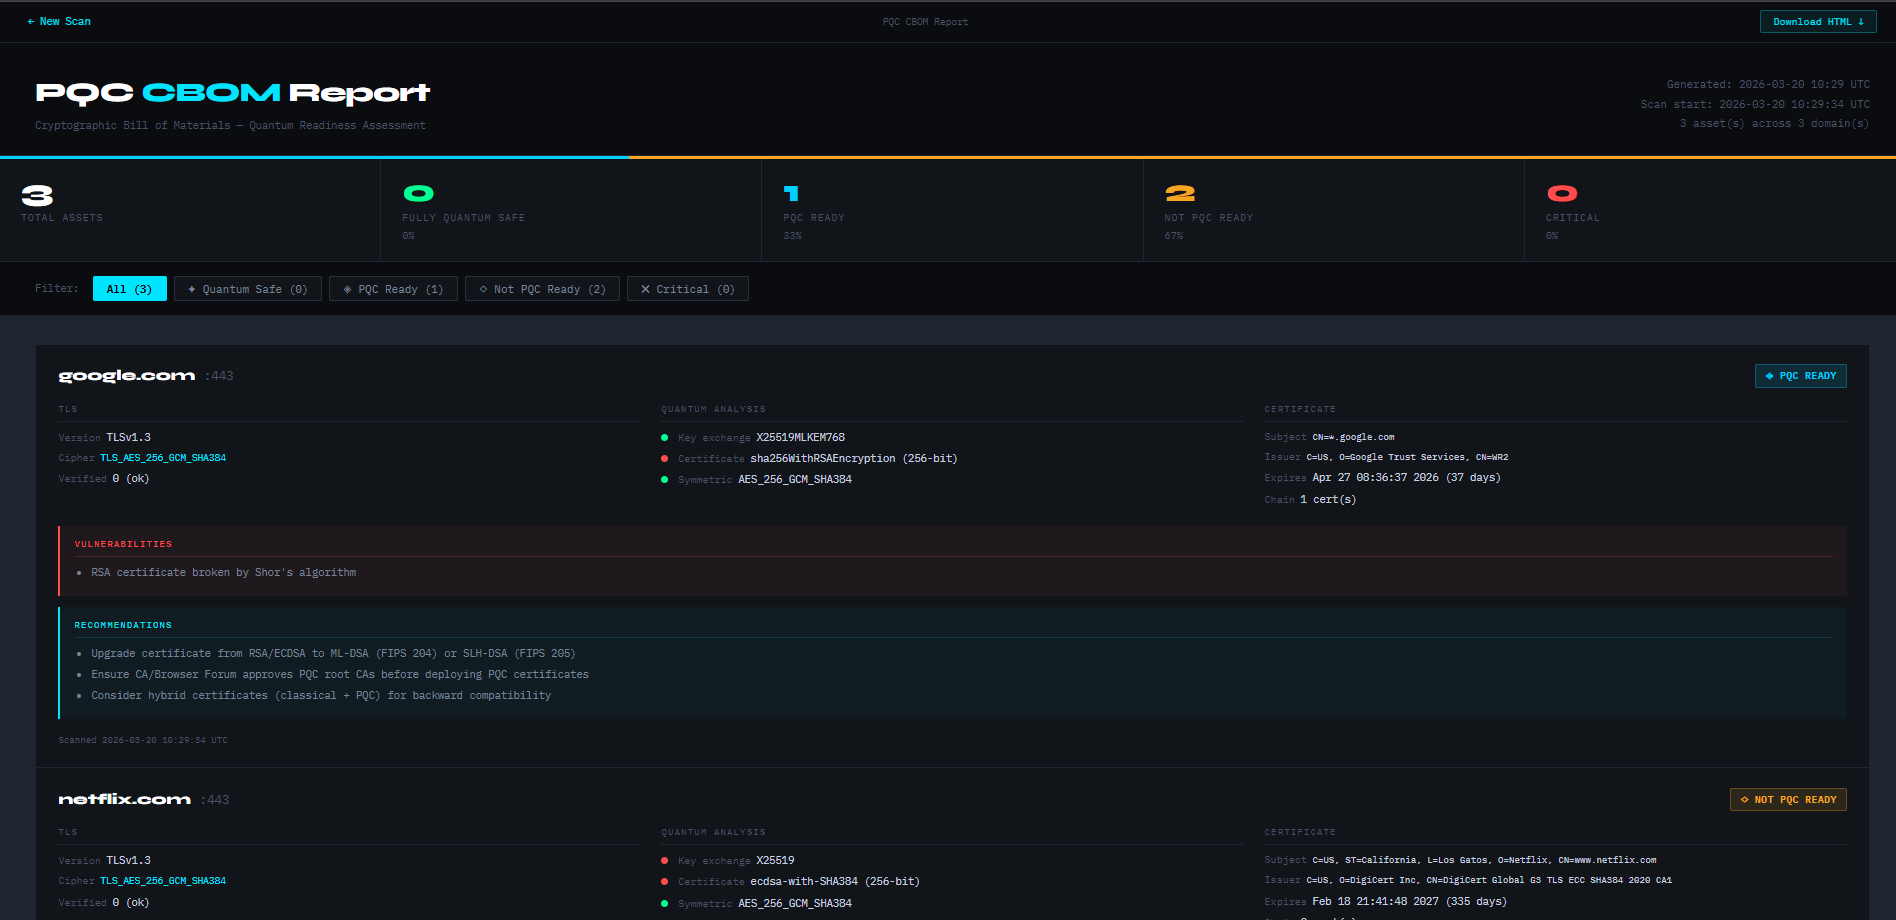
\includegraphics[width=\textwidth]{images/html_report.png}
  \caption{HTML Report — Stats bar, progress bar, and asset cards}
  \label{fig:html_report_overview}
\end{figure}

\begin{reqbox}{FR-6.1 — Self-Contained HTML}
  The generated report \textbf{shall} be a single self-contained HTML file with
  all CSS and JavaScript embedded inline, requiring no internet connection to
  render. \hfill \textbf{[M]}
\end{reqbox}

\begin{reqbox}{FR-6.2 — Summary Statistics}
  The report header \textbf{shall} display total asset count and per-tier count
  with percentage for each of the four quantum readiness labels. \hfill \textbf{[M]}
\end{reqbox}

\begin{reqbox}{FR-6.3 — Visual Progress Bar}
  The report \textbf{shall} render a horizontal progress bar with colour-coded
  segments proportional to the count of each tier, providing an at-a-glance
  portfolio health view. \hfill \textbf{[M]}
\end{reqbox}

\begin{reqbox}{FR-6.4 — Filter Controls}
  The report \textbf{shall} provide interactive filter buttons to show only assets
  matching a selected tier label (All / FQS / PQC / Not PQC / Critical) without
  a page reload. \hfill \textbf{[M]}
\end{reqbox}

\begin{reqbox}{FR-6.5 — Domain Grouping}
  Assets \textbf{shall} be grouped by their root domain (eTLD+1), with subdomains
  displayed in a collapsible drawer beneath the root asset card. \hfill \textbf{[S]}
\end{reqbox}

\begin{reqbox}{FR-6.6 — Asset Card Detail}
  Each asset card \textbf{shall} display:
  \begin{itemize}[noitemsep]
    \item TLS version and cipher suite.
    \item Key exchange algorithm and PQC classification dot.
    \item Certificate subject, issuer, expiry (colour-coded), and chain depth.
    \item Signature algorithm and PQC classification dot.
    \item Symmetric cipher and safety dot.
    \item Vulnerability list.
    \item Recommendation list.
    \item Scan timestamp.
  \end{itemize}
  \hfill \textbf{[M]}
\end{reqbox}

\begin{reqbox}{FR-6.7 — Certificate Expiry Warnings}
  Certificate expiry \textbf{shall} be displayed in:
  \begin{itemize}[noitemsep]
    \item \textcolor{critical}{\textbf{Red}} — certificate already expired.
    \item \textcolor{notpqc}{\textbf{Amber}} — fewer than 30 days remaining.
    \item Normal colour — otherwise.
  \end{itemize}
  \hfill \textbf{[M]}
\end{reqbox}

\begin{reqbox}{FR-6.8 — Report Download}
  The report page \textbf{shall} provide a \textit{Download HTML} button that
  saves the report as a standalone file to the user's local machine. \hfill \textbf{[S]}
\end{reqbox}

% ─────────────────────────────────────────────────────────────────────────────
\section{Feature 7: Web GUI and Real-Time Streaming}
\label{sec:fr_gui}

\begin{figure}[H]
  \centering
  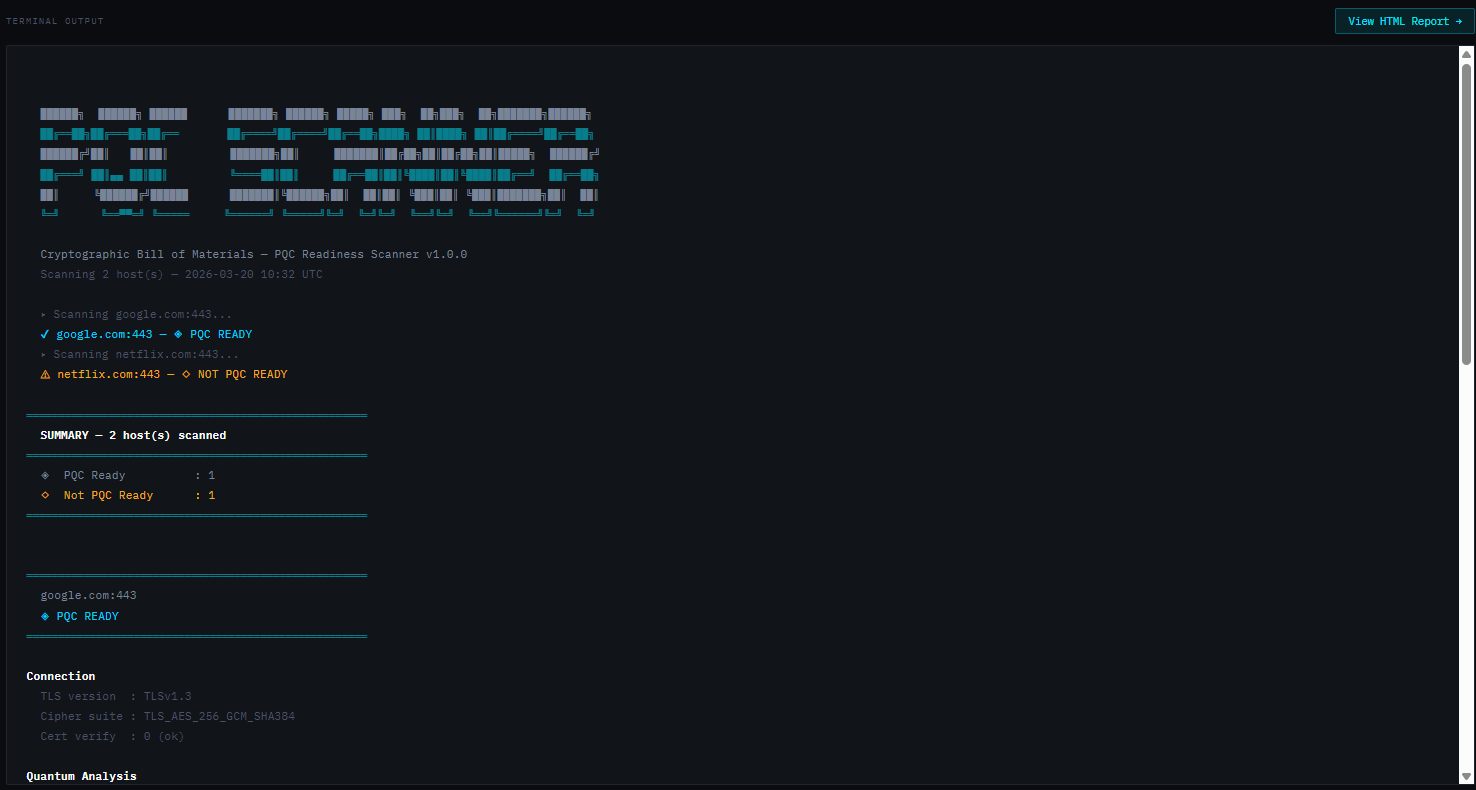
\includegraphics[width=\textwidth]{images/web_terminal_output.png}
  \caption{Web GUI — Terminal output panel with real-time SSE streaming}
  \label{fig:gui_terminal}
\end{figure}

\begin{reqbox}{FR-7.1 — Real-Time Output Streaming}
  The web application \textbf{shall} stream scan output to the browser in real time
  using Server-Sent Events (SSE), rendering each line as it is produced by the
  scanner. \hfill \textbf{[M]}
\end{reqbox}

\begin{reqbox}{FR-7.2 — ANSI Colour Rendering}
  Colour codes emitted by the scanner (\texttt{\\033[...m} sequences)
  \textbf{shall} be converted to appropriate HTML/CSS styling so that tier labels
  appear in their corresponding colours in the browser output panel. \hfill \textbf{[M]}
\end{reqbox}

\begin{reqbox}{FR-7.3 — Scan Status Indicator}
  A spinner or progress indicator \textbf{shall} be visible while a scan is
  running and hidden upon completion. \hfill \textbf{[S]}
\end{reqbox}

\begin{reqbox}{FR-7.4 — Report Link Post-Scan}
  Upon successful scan completion, the GUI \textbf{shall} display a
  \textit{View HTML Report} link that opens the generated report in a new
  browser tab. \hfill \textbf{[M]}
\end{reqbox}

\begin{reqbox}{FR-7.5 — Stop Scan}
  The GUI \textbf{shall} provide a \textit{Stop Scan} button that becomes visible
  during a running scan and, when clicked, sends a SIGTERM to the scanner
  process to terminate it gracefully. \hfill \textbf{[M]}
\end{reqbox}

\begin{reqbox}{FR-7.6 — SSE Keepalive}
  The SSE stream \textbf{shall} emit a keepalive comment every 5 seconds to
  prevent intermediate proxies from closing the connection prematurely.
  \hfill \textbf{[S]}
\end{reqbox}

% ─────────────────────────────────────────────────────────────────────────────
\section{Feature 8: Report Lifecycle Management}
\label{sec:fr_lifecycle}

\begin{reqbox}{FR-8.1 — In-Memory Report Storage}
  Generated reports \textbf{shall} be held in server memory and accessible via a
  unique report identifier for the duration of the configured TTL (default:
  3600 seconds). \hfill \textbf{[M]}
\end{reqbox}

\begin{reqbox}{FR-8.2 — Automatic Report Eviction}
  A background daemon thread \textbf{shall} evict expired reports every 5 minutes
  to prevent unbounded memory growth. \hfill \textbf{[M]}
\end{reqbox}

\begin{reqbox}{FR-8.3 — TTL Configuration}
  The report TTL \textbf{shall} be configurable via the \texttt{REPORT\_TTL}
  environment variable without code changes. \hfill \textbf{[S]}
\end{reqbox}
